\section{\bench: a memory-dependent harvesting benchmark}
\label{sec:benchmark}

\paragraph{Scene, robot and sensing} \bench\ is built on ManiSkill3 \citep{tao2025maniskill3} (environment \texttt{FruitPick-v1}). Each episode samples a tree with a trunk, branches and leaf clusters, and 4--6 spherical fruits of radius 2.5--2.9~cm at heights of 0.44--0.64~m, distances of 0.38--0.50~m from the robot base and within $\pm 28^\circ$ of azimuth. The layout sampler guarantees an inverse-kinematics solution for a horizontal approach, a branch-free approach corridor and no mutual occlusion of fruits in the front camera. A fruit is attached to its stem until it has been held between both fingers for two consecutive control steps; it then becomes a dynamic rigid body. The robot is a RealMan RM75-B 7-DoF arm with an EG2 parallel gripper under joint-position control (a 6-DoF RM65-B is also supported). Observations are a front and a wrist RGB-D camera ($256\times256$ pixels; front field of view $55^\circ$) and an 8-dimensional state (seven joint angles and one finger position); actions are seven absolute joint targets and a gripper command.

\paragraph{Tasks}
\label{sec:tasks}
Figure~\ref{fig:scene} shows both tasks. In \textbf{FruitOccludedRipe}, red (ripe) and green (unripe) fruits hang together. During a 30-step observation phase, a gust between steps 8 and 20 blows two leaf clusters in front of two fruits, at least one of them ripe, so ``hidden'' does not imply ``ripe''. The instruction is to put all ripe fruits into the basket. Leaves are pushed aside when the gripper comes within 15~cm, so the final approach is visible, but \emph{finding} a hidden ripe fruit requires remembering it. Success requires every ripe fruit and no unripe fruit in the basket; a dropped fruit is a failure. In \textbf{FruitCount}, all $M$ fruits are ripe and the instruction asks for exactly $N<M$ of them ($N=2$--5). The basket is outside the front camera view, so the policy can only know how many it has picked by remembering its own picks. Success requires exactly $N$ fruits in the basket; over-picking or dropping is a failure.

\begin{figure}[t]
\centering
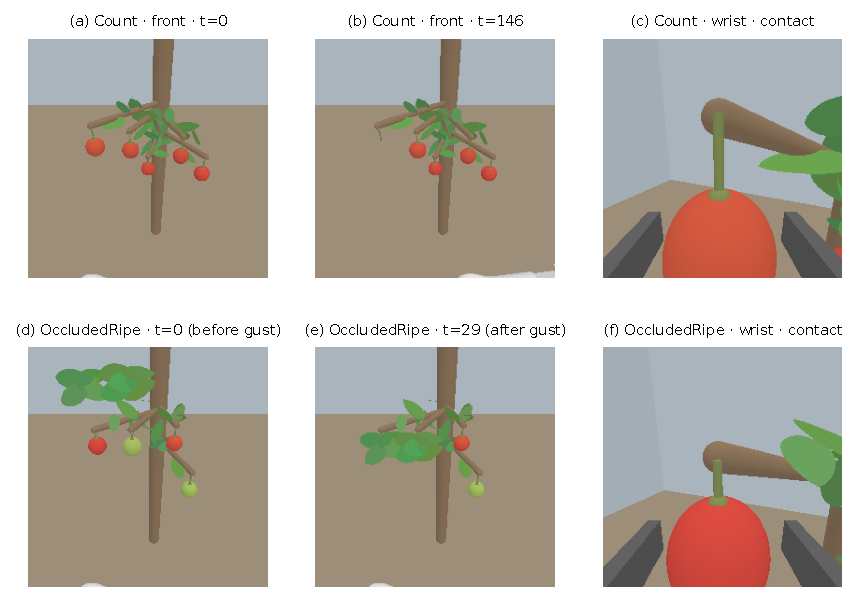
\includegraphics[width=0.78\linewidth]{fig2_scene}
\caption{\bench\ tasks. (a--c) FruitCount: front view at the start and after one pick, and the wrist view at contact. (d--f) FruitOccludedRipe: the front view before and after the wind gust (two leaf clusters now hide fruits) and the wrist view at contact.}
\label{fig:scene}
\end{figure}

\paragraph{Demonstrations} A scripted demonstrator plans with mplib \citep{mplib} through eight phases (observe, reach, approach, grasp, pull, carry, release, settle); failed attempts are discarded, and every frame stores the ground-truth fruit poses and attachment, visible pixels per camera, phase labels and TCP pose. Recovery demonstrations (DART-H, Section~\ref{sec:dart}) use the same demonstrator with execution noise. Table~\ref{tab:dataset} summarizes the 640 demonstrations. After the gust, the targeted fruits are fully invisible in the front camera; over all frames in which an occluded fruit is still on the tree, it is invisible in 72\% of frames on average (median 78\%), and two-thirds of the leaf clusters hide a ripe fruit (Table~S1 in the Supplementary material, with the phase structure).

\begin{table}[t]
\centering
\caption{Benchmark statistics (steps: mean $\pm$ SD). Acceptance: fraction of demonstrator attempts that succeeded. Training features: 88,607 samples (clean) and 173,791 (clean + DART-H).}
\label{tab:dataset}
\footnotesize
\begin{adjustbox}{max width=\textwidth}\begin{tabular}{llrccccc}
\toprule
Set (episodes) & Task & $n$ & Steps & Range & Fruits & Picks & Acceptance\\
\midrule
Clean train (0--99) & FruitCount & 100 & $474\pm124$ & 320--757 & 4.73 & 2.85 & 0.96\\
 & FruitOccludedRipe & 100 & $412\pm85$ & 295--710 & 4.69 & 2.54 & 0.98\\
DART-H train (100--199) & FruitCount & 100 & $455\pm133$ & 314--876 & 4.62 & 2.70 & 0.57\\
 & FruitOccludedRipe & 100 & $397\pm89$ & 297--672 & 4.78 & 2.46 & 0.66\\
Development (200--219) & FruitCount & 20 & $487\pm162$ & 321--766 & 5.05 & 3.10 & 1.00\\
 & FruitOccludedRipe & 20 & $369\pm71$ & 300--471 & 4.60 & 2.35 & 0.95\\
Validation (0--49) & FruitCount & 50 & $459\pm142$ & 314--904 & 4.58 & 2.82 & 0.98\\
 & FruitOccludedRipe & 50 & $396\pm87$ & 300--630 & 4.72 & 2.50 & 0.96\\
Validation (50--99) & FruitCount & 50$^{a}$ & $499\pm169$ & 322--1037 & 4.67 & 2.98 & 0.91\\
 & FruitOccludedRipe & 50 & $392\pm73$ & 304--534 & 4.54 & 2.52 & 0.98\\
\bottomrule
\end{tabular}\end{adjustbox}

\footnotesize $^{a}$Statistics over 49 episodes; the ground-truth file of one episode was regenerated after these statistics were computed.
\end{table}
